% !TeX root = RJwrapper.tex
\title{Fairness Audits and Debiasing Using \pkg{mlr3fairness}}


\author{by Florian Pfisterer, Siyi Wei, Sebastian Vollmer, Michel Lang, and Bernd Bischl}

\maketitle

\abstract{%
Given an increase in data-driven automated decision-making based on machine learning (ML) models, it is imperative that, along with tools to develop and improve such models, there are sufficient capabilities to analyze and assess models with respect to potential biases. We present the package \CRANpkg{mlr3fairness}, a collection of metrics and methods that allow for the assessment of bias in machine learning models. Our package implements a variety of widely used fairness metrics that can be used to audit models for potential biases, along with a set of visualizations that can help to provide additional insights into such biases. \CRANpkg{mlr3fairness} furthermore integrates bias mitigation methods for machine learning models through data pre-processing or post-processing of predictions. These allow practitioners to trade off performance and fairness metrics that are appropriate for their use case.
}

\hypertarget{introduction}{%
\section{Introduction}\label{introduction}}

Humans are increasingly subject to data-driven automated decision-making.
Those automated procedures, such as credit risk assessments, are often applied using predictive models (Kozodoi, Jacob, and Lessmann 2022; Galindo and Tamayo 2000), often profoundly affecting individual's lives.
It is therefore important that, along with tools to develop and improve such models, we also develop sufficient capabilities to analyze and assess models not only with respect to their robustness and predictive performance but also with respect to potential biases.
This is highlighted by the European General Data Protection Regulation (GDPR) which requires data to be processed fairly.
Popular modelling frameworks for the R language (R Core Team 2021) such as \CRANpkg{caret} (Kuhn 2021), \CRANpkg{tidymodels} (Kuhn and Wickham 2020), \CRANpkg{SuperLearner} (Polley et al. 2021), or \CRANpkg{mlr} (Bischl et al. 2016) implement a plethora of metrics to measure performance, but fairness metrics are widely missing.
This lack of availability can be detrimental to obtaining fair and unbiased models if the result is to forgo bias audits due to the considerable complexity of implementing such metrics.
Consequently, there exists a considerable necessity for R packages to (a) implement such metrics, and (b) to connect these metrics to existing ML frameworks.
If biases are detected and need to be mitigated, we might furthermore want to employ bias mitigation techniques that tightly integrate with the fitting and evaluation of the resulting models in order to obtain trade-offs between a model's fairness and utility (e.g., predictive accuracy).

In this article, we present the \CRANpkg{mlr3fairness} package which builds upon the ML framework \CRANpkg{mlr3} (Lang et al. 2019).
Our extension contains fairness metrics, fairness visualizations, and model-agnostic pre- and post-processing operators that aim to reduce biases in ML models.
Additionally, \CRANpkg{mlr3fairness} comes with reporting functionality that assists the user in documenting data and ML models, as well as in performing fairness audits.

In the remainder of the article, we first provide an introduction to fairness in ML to raise awareness of biases that can arise due to the use of ML models.
Next, we introduce the \CRANpkg{mlr3fairness} package, followed by an extensive case study, showcasing the capabilities of \CRANpkg{mlr3fairness}.
We conclude with a summary.

\hypertarget{fairness-in-machine-learning}{%
\section{Fairness in Machine Learning}\label{fairness-in-machine-learning}}

Studies have found that data-driven automated decision-making systems often improve over human expertise (Dawes, Faust, and Meehl (1989)) and high-stakes decisions can therefore be enhanced using data-driven systems.
This often does not only improve predictions, but can also make decisions more efficient through automation.
Such systems, often without human oversight, are now ubiquitous in everyday life (O'neil 2016; Eubanks 2018; Noble 2018).
To provide further examples, ML-driven systems are used for highly influential decisions such as loan accommodations (Chen 2018; Turner and McBurnett 2019), job applications (Schumann et al. 2020), healthcare (Topol 2019), and criminal sentencing (Angwin et al. 2016; Corbett-Davies et al. 2017; Berk et al. 2018).
With this proliferation, such decisions have become subject to scrutiny as a result of prominent inadequacies or failures, for example in the case of the COMPAS recidivism prediction system (Angwin et al. 2016).

Without proper auditing, those models can unintentionally result in negative consequences for individuals, often from underprivileged groups (Barocas, Hardt, and Narayanan 2019).
Several sources of such biases are worth mentioning in this context:
Data often contains \textbf{historical biases} such as gender or racial stereotypes, that -- if picked up by the model -- will be replicated into the future.
Similarly, unprivileged populations are often not represented in data due to \textbf{sampling biases} leading to models that perform well in groups sufficiently represented in the data but worse on others (Buolamwini and Gebru 2018) -- this includes a higher rate of missing data.
Other biases include biases in how \emph{labels} and \emph{data} are measured (Bao et al. 2021) as well as \textbf{feedback} loops where repeated decisions affect the population subject to such decisions.
For an in-depth discussion and further sources of biases, the interested reader is referred to available surveys of the field (Barocas, Hardt, and Narayanan 2019; Mehrabi et al. 2021; S. Mitchell et al. 2021).

\hypertarget{quantifying-fairness}{%
\subsection{Quantifying fairness}\label{quantifying-fairness}}

We now turn to the question of how we can detect whether disparities exist in a model and if so, how they can be quantified.
What constitutes a fair model depends on a society's ethical values and which normative position we take, resulting in different metrics that are applied to a problem at hand.
In this article, we focus on a subgroup of these, so-called \emph{statistical group fairness} metrics.
First, the observations are grouped by a sensitive attribute \(A\) (\(A = 0\) vs.~\(A = 1\)), which, e.g., is an identifier for a person's race or a person's gender.
For the sake of simplicity, we consider a \emph{binary classification} scenario and a \emph{binary sensitive attribute}.
Each observation has an associated label \(Y, Y \in \{0, 1\}\), and we aim to predict, e.g., whether a defendant was caught re-offending.
A system then makes a prediction \(\hat{Y}, \hat{Y} \in \{0,1\}\), with the goal to predict whether an individual might re-offend.
We assume that \(Y = 1\) is the favored outcome in the following exposition.
While we do not describe them in detail, the concepts discussed in the following often extend naturally to more complex scenarios including multi-class classification, regression or survival analysis.
Similarly, metrics can be extended to settings that require consideration of multiple possibly intersecting sensitive attributes.
We now provide and discuss groups of metrics that require either \emph{Separation} or \emph{Independence} (Barocas, Hardt, and Narayanan 2019) to provide further intuition regarding core concepts and possible applications.

\hypertarget{separation}{%
\subsubsection{Separation}\label{separation}}

One group of widely used fairness notions requires \textbf{Separation}: \(\hat{Y} \perp A | Y\).
In order for separation to hold, the prediction \(\hat{Y}\) has to be independent of \(A\) given the true label \(Y\).
This essentially requires that some notion of model error, e.g., accuracy or false positive rate, is equal across groups \(A\).
From this notion, we can derive several metrics that come with different implications.
It is important to note that those metrics can only meaningfully identify biases under the assumption that no disparities exist in the data or that they are legally justified.
For example, if societal biases lead to disparate measurements of an observed quantity (e.g.~SAT scores) for individuals with the same underlying ability, \emph{separation} based metrics might not identify existing biases.
For this reason, Wachter, Mittelstadt, and Russell (2020) refer to those metrics as \emph{bias-preserving} metrics since underlying disparities are not addressed.

\hypertarget{equalized-odds}{%
\paragraph{Equalized Odds}\label{equalized-odds}}

A predictor \(\hat{Y}\) satisfies \emph{equalized odds} with respect to a sensitive attribute \(A\) and observed outcome \(Y\), if \(\hat{Y}\) and \(A\) are conditionally independent given \(Y\):
\begin{equation}
\mathbb{P}\left(\hat{Y} = 1 \mid A = 0, Y = y\right) = \mathbb{P}\left(\hat{Y} = 1 \mid A = 1, Y = y\right), \quad y \in \{0,1\}.
\label{eq:eod}
\end{equation}
In short, we require that the true positive rates (TPR) and false positive rates (FPR) across both groups \(A = 0\) and \(A = 1\) are equal.
This intuitively requires, e.g., in the case of university admission, independent of the sensitive attribute, equal chances for qualified individuals to be accepted and unqualified individuals to be rejected.
Similar measures have been proposed based on equalized false positive rates (Chouldechova 2017) and false omission rates (Berk et al. 2018), depending on the scenario and societal context.

\hypertarget{equality-of-opportunity}{%
\paragraph{Equality of Opportunity}\label{equality-of-opportunity}}

A predictor \(\hat{Y}\) satisfies \emph{equality of opportunity} with respect to a sensitive attribute \(A\) and observed outcome \(Y\), if \(\hat{Y}\) and \(A\) are conditionally independent for \(Y = 1\).
This is a relaxation of the aforementioned \emph{equalized odds} essentially only requiring equal TPRs:
\begin{equation}
\mathbb{P}\left(\hat{Y} = 1 \mid A = 0, Y = 1\right) = \mathbb{P}\left(\hat{Y} = 1 \mid A = 1, Y = 1\right).
\label{eq:eop}
\end{equation}
Intuitively, this only requires that, independent of the sensitive attribute, qualified individuals have the same chance of being accepted.

\hypertarget{performance-parity}{%
\paragraph{Performance Parity}\label{performance-parity}}

A more general formulation can be applied when we require parity of some performance metric across groups.
To provide an example, Buolamwini and Gebru (2018) compare accuracy across intersectional subgroups, essentially arguing that model performance should be equal across groups:

\begin{equation}
\mathbb{P}\left(\hat{Y} = Y \mid A = 0\right) = \mathbb{P}\left(\hat{Y} = Y \mid A = 1\right).
 \label{eq:accp}
\end{equation}
This intuitively requires that the model should work equally well for all groups, i.e., individuals are correctly accepted or denied at the same rate, independent of the predicted attribute.
This notion can be extended across supervised learning settings and performance metrics, leading to considerations of equal mean squared error, e.g., in a regression setting.

\hypertarget{independence}{%
\subsubsection{Independence}\label{independence}}

The second group of fairness metrics is given by so-called \emph{bias-transforming} metrics (Wachter, Mittelstadt, and Russell 2020).
They require that decision rates, such as the positive rate, are equal across groups.
This notion can identify biases, e.g., those which arise from societal biases, that manifest in different base rates across groups.
At the same time, employing such notions poses a considerable risk, as blindly optimizing for demographic parity might result in predictors that, for example jail innocent people from an advantaged group in order to achieve parity across both groups (Dwork et al. 2012; Berk et al. 2018).
A predictor \(\hat{Y}\) satisfies \emph{demographic parity} (Calders and Verwer 2010) with respect to a sensitive attribute \(A\) and observed outcome \(Y\), if \(\hat{Y}\) and \(A\) are conditionally independent:
\begin{equation}
\mathbb{P}\left(\hat{Y} = 1 \mid A = 0\right) = \mathbb{P}\left(\hat{Y} = 1 \mid A = 1\right).
 \label{eq:dp}
\end{equation}
In contrast to the previous definitions, this requires that the chance of being accepted is equal across groups.

\hypertarget{fairness-metrics}{%
\subsubsection{Fairness metrics}\label{fairness-metrics}}

In order to encode the requirements in equations \eqref{eq:eod} - \eqref{eq:dp} into a fairness metric, we encode differences between measured quantities in two groups.
For a performance metric \(M\), e.g., the true positive rate (TPR), we calculate the difference in the metric across the two groups:

\[
\Delta_{\mathrm{M}} = \mathrm{M}_{A=0} - \mathrm{M}_{A=1}.
\]
When \(\Delta_{\mathrm{M}}\) significantly deviates from \(0\), this indicates a fairness violation with respect to the fairness notion described in \(M\).
To provide an example, with \(\mathbb{P}\left(\hat{Y} = 1 \mid A = \star, Y = 1\right)\) denoted with \(\mathrm{TPR}_{A=\star}\), we calculate the difference in TPR between the two groups:
\[
\Delta_{\mathrm{TPR}} = \mathrm{TPR}_{A=0} - \mathrm{TPR}_{A=1}.
\]
When \(\Delta_{\mathrm{TPR}}\) now significantly deviates from \(0\), the prediction \(\hat{Y}\) violates the requirement for \emph{equality of opportunity} formulated above.

It is important to note that in practice, we might not be able to perfectly satisfy a given metric, e.g., due to stochasticity in data and labels.
Instead, to provide a binary conclusion regarding fairness, a model could be considered fair if \(|\Delta_{\mathrm{TPR}}| < \epsilon\) for a given threshold \(\epsilon > 0\), e.g., \(\epsilon = 0.05\).
This allows for small deviations from perfect fairness due to variance in the estimation of \(\mathrm{TPR}_{A=\star}\) or additional sources of bias.
However, choosing appropriate thresholds is difficult, and widely used values for \(\epsilon\) such as \(0.05\) are arbitrary and do not translate to legal doctrines, e.g., disparate impact (Watkins, McKenna, and Chen 2022).
A more in-depth treatment of metrics is given by (Barocas, Hardt, and Narayanan 2019; Saleiro et al. 2018; Kim, Chen, and Talwalkar 2020; Mehrabi et al. 2021; Wachter, Mittelstadt, and Russell 2020).

\hypertarget{selecting-fairness-metrics}{%
\paragraph{Selecting fairness metrics}\label{selecting-fairness-metrics}}

While the aforementioned metrics are conceptually similar, they encode different beliefs of what constitutes \emph{fair} in a given scenario.
Wachter, Mittelstadt, and Russell (2020) differentiate between \emph{bias-preserving} and \emph{bias-transforming} metrics:
Bias-preserving metrics such as equalized odds and equality of opportunity require that errors made by a model are equal across groups.
This can help to detect biases stemming, from imbalances in the sampling or under- and overfitting in ML models, but might be problematic in cases where labels are biased.
To provide an example, police enforcement and subsequent arrests of violent re-offenders might be different across ZIP code areas, a proxy for race.
This might lead to situations where observed labels \(Y\) suffer from differential measurement bias strongly correlated with race (Bao et al. 2021).
Bias-preserving metrics do not take such disparities into account and might, therefore (wrongly) lead to the conclusion that a given model is fair.

Bias-transforming methods, in contrast, do not depend on labels and might therefore not suffer from this problem.
They can help detect biases arising from different base rates across populations, arising, e.g., from aforementioned biases in the labelling or as a consequence of structural discrimination.
Deciding which metrics to use constitutes a value judgement and requires careful assessment of the societal context a decision-making system is deployed in.
A discussion of different metrics and their applicability can be found in the Aequitas Fairness Toolkit (Saleiro et al. 2018) which also provides guidance towards selecting a metric via the \href{http://www.datasciencepublicpolicy.org/our-work/tools-guides/aequitas/}{Aequitas Fairness Tree}.
Wachter, Mittelstadt, and Russell (2020) recommend using \emph{bias-transforming} metrics and provide a checklist that can guide the choice of fairness metric.
Corbett-Davies and Goel (2018), on the other hand, point out several limitations of available metrics and argue for grounding decisions in real-world quantities in addition to abstract fairness metrics.
Similarly, Friedler, Scheidegger, and Venkatasubramanian (2016) emphasize the need to differentiate between constructs we aim to measure (e.g., job-related knowledge) and the observed quantity that can be measured in practice (e.g., years in a job) when trying to automate decisions, since disparities in how constructs translate to observed quantities might suffer from bias.
To provide an example, individuals with similar abilities might exhibit different measured quantities (grades) due to structural bias, e.g., differential access to after-school tutoring programs.

\hypertarget{the-dangers-of-fairness-metrics}{%
\paragraph{The dangers of fairness metrics}\label{the-dangers-of-fairness-metrics}}

We want to stress that overly trusting in metrics can be dangerous and that fairness metrics cannot and should not be used to \emph{prove} or \emph{guarantee} fairness.
Whether a selected fairness notion (and a corresponding numerical value) is actually fair depends on the societal context in which a decision is made and which action should be derived from a given prediction.
Therefore, selecting the correct fairness metric requires a thorough understanding of the societal context of a decision, as well as the possible implications of such decisions.
To provide an example, in some cases discrepancies in positive predictions might be justified or even desired, as they, for example, allow for a more nuanced, gender-specific diagnosis (Cirillo et al. 2020).
Furthermore, fairness metrics might not detect biases in more fine-grained subgroups, e.g., at the intersection of multiple sensitive attributes.
It is also important to note that fairness metrics merely provide a reduction of the aforementioned fairness notions into mathematical objectives.
As such, they require a variety of abstraction steps that might invalidate the metric (Watkins, McKenna, and Chen 2022), as they, for example, require that the data is a large enough and representative sample of exactly the population that we aim to investigate.
Furthermore, practitioners need to look beyond the model, and also at the data used for training and the process of data and label acquisition.
If the data for example exhibit disparate measurement errors in the features or labels, valid fairness assessments can become impossible.
Similarly, feedback loops might arise from a prediction leading to changes in the data collected in the future.
Even an \emph{initially fair} model might then lead to adverse effects in the long term (Schwöbel and Remmers 2022).

Note that the fairness definitions presented above serve a dual purpose (Wachter, Mittelstadt, and Russell 2020):
First, as a \emph{diagnostic tool} to detect disparities.
This allows for assessing whether a model has inherited biases, e.g., from historical disparities reflected in the data.
The second purpose is as a basis for \emph{model selection} and making fair decisions in practice.
In this setting, fairness notions are employed to audit ML models or to select which model should be used in practice.
In this setting, it is important to note that fairness metrics should not be used as the sole basis for making decisions about whether to employ a given ML model or to assess whether a given system is fair.
We therefore explicitly encourage using the presented metrics for exploratory purposes.

\hypertarget{other-notions-of-fairness}{%
\paragraph{Other notions of fairness}\label{other-notions-of-fairness}}

In addition to \emph{statistical group fairness notions} introduced above, several additional fairness notions exist.
The notion of \emph{individual fairness} was proposed by Dwork et al. (2012).
Its core idea comes from the principle of \emph{treating similar cases similarly and different cases differently}.
In contrast to statistical group fairness notions, this notion allows assessing \emph{fairness} at an individual level and
would therefore allow determining whether an individual is treated fairly.
A more in-depth treatment of individual fairness notions is, given in Binns (2020).
Similarly, a variety of \emph{causal} fairness notions exist (c.f. Kilbertus et al. (2017)).
They argue that assessing fairness requires incorporating causal relationships in the data and propose a variety of causal fairness metrics based on a \emph{directed acyclic graph} describing relationships in the data.

\hypertarget{fairness-constraints}{%
\paragraph{Fairness constraints}\label{fairness-constraints}}

Statistical group fairness notions suffer from two further problems in practice:
First, it might be hard to exactly satisfy the required fairness notions, e.g., due to a limited amount of data available for evaluation.
Secondly, only requiring fairness might lead to degenerate solutions (Corbett-Davies and Goel 2018) or models that have low utility, e.g., in separating \emph{good} and \emph{bad} credit risk.
One approach to take this into account is to employ models which maximize utility but satisfy some maximum constraint on potential unfairness.
This can be achieved via constraints on the employed fairness measure, e.g.~\(|\Delta_M| \leq \epsilon\) requiring that the absolute difference in a metric \(M\) between groups
is smaller than a chosen value \(\epsilon\).
In the following, we denote the fairness metric we want to minimize with \(\Delta_M\) and a performance metric with \(\rho\).

\[
  \rho_{|\Delta_M| \leq \epsilon} = \left\{
\begin{array}{ll}
\rho         & |\Delta_M| \leq \epsilon      \\
- |\Delta_M| &  \textrm{else.}                \\
\end{array}
\right.
\]

Note that this assumes that the fairness metric \(\rho\) is strictly positive and should be maximized.
This approach is similar in spirit to the approach of Perrone et al., (2021) who optimize the constrained expected improvement \(cEI = \mathbb{P}(|\Delta_M| \leq \epsilon) \cdot \rho\).

However, it is not immediately clear how the constraint \(\epsilon\) should be chosen.
An alternative, therefore, is to employ \emph{multi-objective optimization} to investigate available trade-offs between performance and accuracy metrics.
This can be done via \CRANpkg{mlr3tuning} (Becker, Lang, et al. 2023) which contains functionality to tune models for multiple metrics, described in more detail in the \href{https://mlr3book.mlr-org.com/optimization.html\#mult-measures-tuning}{mlr3book} (Bernd Bischl 2024).
The result of multi-objective optimization then is the \emph{Pareto-set}: A list of models which optimally trade off the specified objectives.

\hypertarget{bias-mitigation}{%
\subsection{Bias mitigation}\label{bias-mitigation}}

If biases are detected in a model, we might now be interested in improving models in order to potentially mitigate such biases.
Bias in models might arise from a variety of sources, so a careful understanding of the data, data quality and distribution might lead to approaches that can help in decreasing biases, e.g.~through the collection of better or additional data or a better balancing of sensitive groups.
Similarly, biases might arise from the model, through under- or overfitting and more careful tuning of model hyperparameters might help with improving fairness.
Especially if the goal is to satisfy \emph{bias-transforming} metrics, a better solution might often be to address fairness problems in the real world instead of relying on algorithmic interventions to solve fairness. This might lead to more robust, long-term solutions instead of temporarily addressing issues via algorithmic interventions.
In addition, a variety of algorithmic bias mitigation techniques, that might help with obtaining fairer models have been proposed.
Their goal is to reduce measured gaps in fairness, either via data pre-processing, employing models that incorporate fairness, or by applying post-processing techniques to a model's predictions.
Popular examples of such techniques include computing instance weights before training (Kamiran and Calders 2012), where each observation is weighted proportional to the inverse frequency of its label and sensitive attribute.
Other methods work by directly learning fair models that incorporate fairness constraints into the fitting procedure (Zafar et al. 2017) or by adapting model predictions, e.g., Hardt, Price, and Srebro (2016) propose to randomly flip a small fraction of predictions in each group given by \(\hat{Y}\) and \(A\), such that fairness metrics are satisfied in expectation.
Since bias mitigation techniques are often tailored towards a particular fairness metric, the optimal choice is often not trivial and a combination of algorithms and bias mitigation techniques determined via tuning might result in an optimal model.

Bias-mitigation techniques, as proposed above, have the goal of mitigating fairness issues, as measured by fairness metrics.
In practice, this usually comes with several drawbacks:
First, bias-mitigation strategies often lead to a decrease in a classifier's predictive performance (Corbett-Davies and Goel 2018).
In addition, processing schemes can worsen interpretability or introduce stochasticity during prediction (see, e.g., Hardt, Price, and Srebro (2016)).
Furthermore, we want to caution against favouring bias-mitigation techniques over policy interventions that tackle biases at their root cause.
A different set of risks is posed by \emph{fairwashing} (Aivodji et al. 2019), i.e., finding fair explanations or satisfying fairness metrics for otherwise unfair models.
If biases are only addressed at a given moment and without regard for downstream effects, they might simultaneously lead to a decrease in predictive performance in the near term and to negative consequences for the sensitive group in the long term (Schwöbel and Remmers 2022).

\hypertarget{main}{%
\section{\texorpdfstring{The \pkg{mlr3fairness} package}{The  package}}\label{main}}

In this section, we first give an overview of related software.
Next, we give a very brief introduction to the \CRANpkg{mlr3} ecosystem of packages.
Finally, the implemented extensions for fairness are presented.

\hypertarget{related}{%
\subsection{Related software}\label{related}}

Several R packages provide similar capabilities to our software, but mostly focus on fairness metrics and visualization.
The \CRANpkg{fairness} package (Kozodoi and V. Varga 2021) allows for the calculation of a variety of fairness metrics, while \CRANpkg{aif360} (Bellamy et al. 2019) wraps the Python \pkg{aif360} module allowing for the computation of fairness metrics and several bias mitigation techniques, but has only limited interoperability with R objects such as \code{data.frame}s.
The \CRANpkg{fairmodels} (Wiśniewski and Biecek 2022) package again allows for the computation of fairness metrics for classification and regression settings as well as several bias mitigation techniques.
It tightly integrates with \CRANpkg{DALEX} (Biecek 2018) to gain further insight using interpretability techniques.

Outside R, in Python, the \pkg{fairlearn} module (Bird et al. 2020) provides ample functionality to study a wide variety of metrics, bias mitigation with respect to a variety of pre-, in- and post-processing methods as well as to visualize differences.
It furthermore provides a \emph{fairlearn dashboard} providing a comprehensive fairness report.
The \pkg{aif360} (Bellamy et al. 2019) module similarly provides metrics as well as bias mitigation techniques while the \pkg{aequitas} fairness toolkit (Saleiro et al. 2018) provides similar capabilities.
Interoperability with the \pkg{scikit-learn} (Pedregosa et al. 2011) ML framework allows for bias mitigation for a wide variety of ML models in all aforementioned systems.
Similar capabilities are also available in Julia's \pkg{Fairness.jl} (Agrawal, Chen, et al. 2020) library.

\hypertarget{mlr3}{%
\subsection{The mlr3 ecosystem}\label{mlr3}}

\CRANpkg{mlr3fairness} is tightly integrated into the ecosystem of packages around the ML framework \CRANpkg{mlr3} (Lang et al. 2019).
\CRANpkg{mlr3} provides the infrastructure to fit, resample, and evaluate over 100 ML algorithms using a unified API.
Packages from the ecosystem can be installed and updated via the \CRANpkg{mlr3verse} (Lang and Schratz 2023) package.
Multiple extension packages bring numerous additional advantages and extra functionality.
In the context of fairness, the following extension packages deserve special mention:

\begin{itemize}
\tightlist
\item
  \CRANpkg{mlr3pipelines} (Binder et al. 2021) for pre- and postprocessing via pipelining.
  This allows composing bias mitigation techniques with arbitrary ML algorithms shipped with \CRANpkg{mlr3} as well as fusing ML algorithms with pre-processing steps such as imputation or class balancing.
  It furthermore integrates with \CRANpkg{mcboost} (Pfisterer et al. 2021), which implements additional bias mitigation methods.
  We present an example in the supplementary material.
\item
  \CRANpkg{mlr3tuning} and \CRANpkg{bbotk} (Becker, Richter, et al. 2023) for its extensive tuning capabilities.
\item
  \pkg{mlr3proba} (Sonabend et al. 2021) for survival analysis.
\item
  \CRANpkg{mlr3benchmark} for post-hoc analysis of benchmarked approaches.
\item
  \CRANpkg{mlr3oml} as a connector to OpenML (Vanschoren et al. 2014), an online scientific platform for collaborative ML.
\end{itemize}

In order to provide the required understanding for \CRANpkg{mlr3}, we briefly introduce some terminology and syntax.
A full introduction can be found in the mlr3 book (Bernd Bischl 2024).

A \texttt{Task} in \CRANpkg{mlr3} is a basic building block holding the data, storing covariates and the target variable along with some meta-information.
The shorthand constructor function \texttt{tsk()} can be used to quickly access example tasks shipped with \CRANpkg{mlr3} or \CRANpkg{mlr3fairness}.
In the following chunk, we retrieve the binary classification task with id \texttt{"adult\_train"} from the package.
It contains a part of the \texttt{Adult} data set (Dua and Graff 2017).
The task is to predict whether an individual earns more than \$50.000 per year.
The column \texttt{"sex"} is set as a binary sensitive attribute with levels \texttt{"Female"} and \texttt{"Male"}.

\begin{verbatim}
library("mlr3verse")
library("mlr3fairness")

task = tsk("adult_train")
print(task)
\end{verbatim}

\begin{verbatim}
#> <TaskClassif:adult_train> (30718 x 13)
#> * Target: target
#> * Properties: twoclass
#> * Features (12):
#>   - fct (7): education, marital_status, occupation, race, relationship,
#>     sex, workclass
#>   - int (5): age, capital_gain, capital_loss, education_num,
#>     hours_per_week
#> * Protected attribute: sex
\end{verbatim}

The second building block is the \texttt{Learner}.
It is a wrapper around an ML algorithm, e.g., an implementation of logistic regression or a decision tree.
It can be trained on a \texttt{Task} and used for obtaining a \texttt{Prediction} on an independent test set which can subsequently be scored using a \texttt{Measure} to get an estimate for the predictive performance on new data.
The shorthand constructors \texttt{lrn()} and \texttt{msr()} allow for the instantiation of implemented \texttt{Learner}s and \texttt{Measure}s, respectively.
In the following example, we will first instantiate a learner, then split our data into a train and test set, afterwards train it on the train set of the dataset and finally evaluate predictions on held-out test data.
The train-test split in this case is given by row indices, here stored in the \texttt{idx} variable.

\begin{verbatim}
learner = lrn("classif.rpart", predict_type = "prob")
idx = partition(task)
learner$train(task, idx$train)
prediction = learner$predict(task, idx$test)
\end{verbatim}

We then employ the \texttt{classif.acc} measure which measures the accuracy of a prediction compared to the true label:

\begin{verbatim}
measure = msr("classif.acc")
prediction$score(measure)
\end{verbatim}

\begin{verbatim}
#> classif.acc 
#>      0.8382
\end{verbatim}

In the example above, we obtain an accuracy score of 0.8382, meaning our ML model correctly classifies roughly 84 \% of the samples in the test data.
As the split into training set and test set is stochastic, the procedure should be repeated multiple times for smaller datasets (Bischl et al. 2012) and the resulting performance values should be aggregated.
This process is called resampling, and can easily be performed with the \texttt{resample()} function, yielding a \texttt{ResampleResult} object.
In the following, we employ 10-fold cross-validation as a resampling strategy:

\begin{verbatim}
resampling = rsmp("cv", folds = 10)
rr = resample(task, learner, resampling)
\end{verbatim}

We can call the \texttt{aggregate} method on the \texttt{ResampleResult} to obtain the accuracy aggregated across all \(10\) replications.

\begin{verbatim}
rr$aggregate(measure)
\end{verbatim}

\begin{verbatim}
#> classif.acc 
#>      0.8408
\end{verbatim}

Here, we obtain an accuracy of 0.8408, so slightly higher than previous scores, due to using a larger fraction of the data.
Furthermore, this estimate has a lower variance (as it is an aggregate) at the cost of additional computation time.
To properly compare competing modelling approaches, candidates can be benchmarked against each other using the \texttt{benchmark()} function (yielding a \texttt{BenchmarkResult}).
In the following, we compare the decision tree from above to a logistic regression model.
To do this, we use the \texttt{benchmark\_grid} function to compare the two \texttt{Learners} across the same \texttt{Task} and resampling procedure.
Finally, we aggregate the measured scores each learner obtains on each cross-validation split using the \texttt{\$aggregate()} function.

\begin{verbatim}
learner2 = lrn("classif.log_reg", predict_type = "prob")

grid = benchmark_grid(task, list(learner, learner2), resampling)
bmr = benchmark(grid)

bmr$aggregate(measure)[, .(learner_id, classif.acc)]
\end{verbatim}

\begin{verbatim}
#>         learner_id classif.acc
#> 1:   classif.rpart      0.8408
#> 2: classif.log_reg      0.8467
\end{verbatim}

After running the benchmark, we can again call \texttt{.\$aggregate} to obtain aggregated scores.
The \CRANpkg{mlr3viz} package comes with several ready-made visualizations for objects from \texttt{mlr3} via \CRANpkg{ggplot2}'s (Wickham 2016) \texttt{autoplot} function.
For a \texttt{BenchmarkResult}, the \texttt{autoplot} function provides a Box-plot comparison of performances across the cross-validation folds for each \texttt{Learner}.
Figure \ref{fig:bmrbox} contains the box-plot comparison.
We can see that \texttt{log\_reg} has higher accuracy and lower interquartile range across the 10 folds, and we might therefore want to prefer the \texttt{log\_reg} model.

\begin{figure}

{\centering 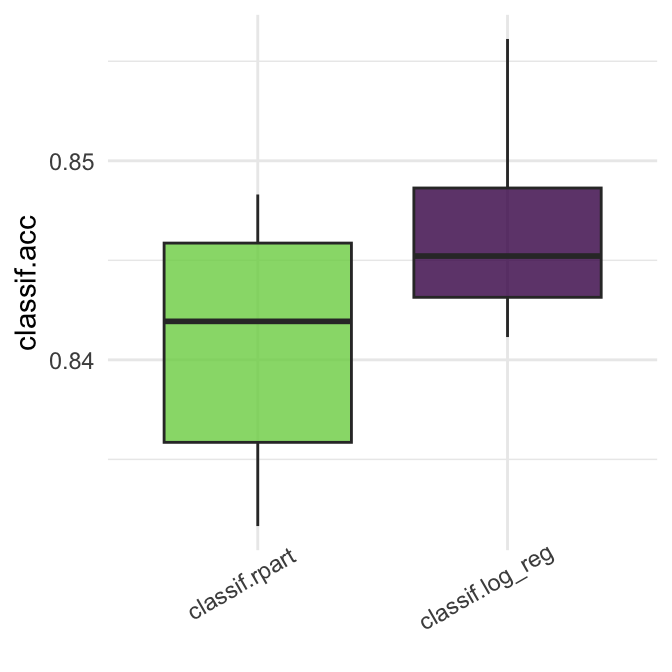
\includegraphics{RJ-2023-034_files/figure-latex/bmrbox-1} 

}

\caption{Model comparison based on accuracy for decision trees (rpart) and logistic regression (log\_reg) across resampling splits.}\label{fig:bmrbox}
\end{figure}

\hypertarget{selecting-the-sensitive-attribute}{%
\subsubsection{Selecting the sensitive attribute}\label{selecting-the-sensitive-attribute}}

For a given task, we can select one or multiple sensitive attributes.
In \CRANpkg{mlr3}, the sensitive attribute is identified by the column role \texttt{pta} and can be set as follows:

\begin{verbatim}
task$set_col_roles("marital_status", add_to = "pta")
\end{verbatim}

In the example above, we add the \texttt{"marital\_status"} as an additional sensitive attribute.
This information is then automatically passed on when the task is used, e.g., when computing fairness metrics.
If more than one sensitive attribute is specified, metrics will be computed based on intersecting groups formed by the columns.

\hypertarget{quantifying-fairness-1}{%
\subsubsection{Quantifying fairness}\label{quantifying-fairness-1}}

With the \CRANpkg{mlr3fairness} package loaded, fairness measures can be constructed via \texttt{msr()} like any other measure in \CRANpkg{mlr3}.
They are listed with prefix \emph{fairness}, and simply calling \texttt{msr()} without any arguments will return a list of all available measures.
Table \ref{tab:metrics} provides an overview of some popular fairness measures which are readily available.

\begin{longtable}[]{@{}
  >{\raggedright\arraybackslash}p{(\columnwidth - 2\tabcolsep) * \real{0.1913}}
  >{\raggedright\arraybackslash}p{(\columnwidth - 2\tabcolsep) * \real{0.8087}}@{}}
\caption{\label{tab:metrics} Overview of fairness metrics available with mlr3fairness.}\tabularnewline
\toprule\noalign{}
\begin{minipage}[b]{\linewidth}\raggedright
key
\end{minipage} & \begin{minipage}[b]{\linewidth}\raggedright
description
\end{minipage} \\
\midrule\noalign{}
\endfirsthead
\toprule\noalign{}
\begin{minipage}[b]{\linewidth}\raggedright
key
\end{minipage} & \begin{minipage}[b]{\linewidth}\raggedright
description
\end{minipage} \\
\midrule\noalign{}
\endhead
\bottomrule\noalign{}
\endlastfoot
fairness.acc & Accuracy equality \citep{gendershades} \\
fairness.mse & Mean squared error equality (Regression) \\
fairness.eod & Equalized odds \citep{hardt2016equality} \\
fairness.tpr & True positive rate equality / Equality of opportunity \citep{hardt2016equality} \\
fairness.fpr & False positive rate equality / Predictive equality \citep{chouldechova2017fair} \\
fairness.tnr & True negative rate equality \\
fairness.fnr & False negative rate equality \citep{richardcompas} \\
fairness.fomr & False omission rate equality \citep{richardcompas} \\
fairness.tnr & Negative predictive value equality \\
fairness.tnr & Positive predictive value equality \\
fairness.cv & Demographic parity / Equalized positive rates \citep{Calders2010} \\
fairness.pp & Predictive parity / Equalized precision \citep{chouldechova2017fair} \\
fairness.\{tp, fp, tn, fn\} & Equal true positives, false positives, true negatives, false negatives \\
fairness.acc\_eod=.05 & Accuracy under equalized odds constraint \citep{perrone2021fair} \\
fairness.acc\_ppv=.05 & Accuracy under ppv constraint \citep{perrone2021fair} \\
\end{longtable}

Furthermore, new custom fairness measures can be easily implemented, either by implementing them directly or by composing them from existing metrics.
This process is extensively documented in an accompanying \href{https://mlr3fairness.mlr-org.com/articles/measures-vignette.html}{measures vignette} available with the package.

Here we choose the binary accuracy measure \texttt{"classif.acc"} and the equalized odds metric from above using \texttt{"fairness.eod"}:
The constructed list of measures can then be used to score a \texttt{Prediction}, a \texttt{ResampleResult} or \texttt{BenchmarkResult}, e.g.

\begin{verbatim}
measures = list(msr("classif.acc"), msr("fairness.eod"))
rr$aggregate(measures)
\end{verbatim}

\begin{verbatim}
#>             classif.acc fairness.equalized_odds 
#>                 0.84078                 0.07939
\end{verbatim}

We can clearly see a comparatively large difference in equalized odds at around 0.08.
This means, that in total, the false positive rates (FPR) and true positive rates (TPR) on average differ by \textasciitilde0.08, indicating that our model might exhibit a bias.
Looking at the individual components yields a clearer picture.
Here, we are looking at the confusion matrices of the combined predictions of the 10 folds, grouped by sensitive attribute:

\begin{verbatim}
fairness_tensor(rr)
\end{verbatim}

\begin{verbatim}
#> $Male
#>         truth
#> response   <=50K    >50K
#>    <=50K 0.43030 0.10033
#>    >50K  0.03408 0.11202
#> 
#> $Female
#>         truth
#> response    <=50K     >50K
#>    <=50K 0.282668 0.020900
#>    >50K  0.003907 0.015789
\end{verbatim}

Plotting the prediction density or comparing measures graphically often provides additional insights:
For example, in Figure \ref{fig:predplots}, we can see that Females are more often predicted to earn below \$50.000.
Similarly, we can see that both equality in FPR and TPR differ considerably.

\begin{verbatim}
fairness_prediction_density(prediction, task)
compare_metrics(prediction, msrs(c("fairness.fpr", "fairness.tpr", "fairness.eod")), task)
\end{verbatim}

\begin{figure}

{\centering 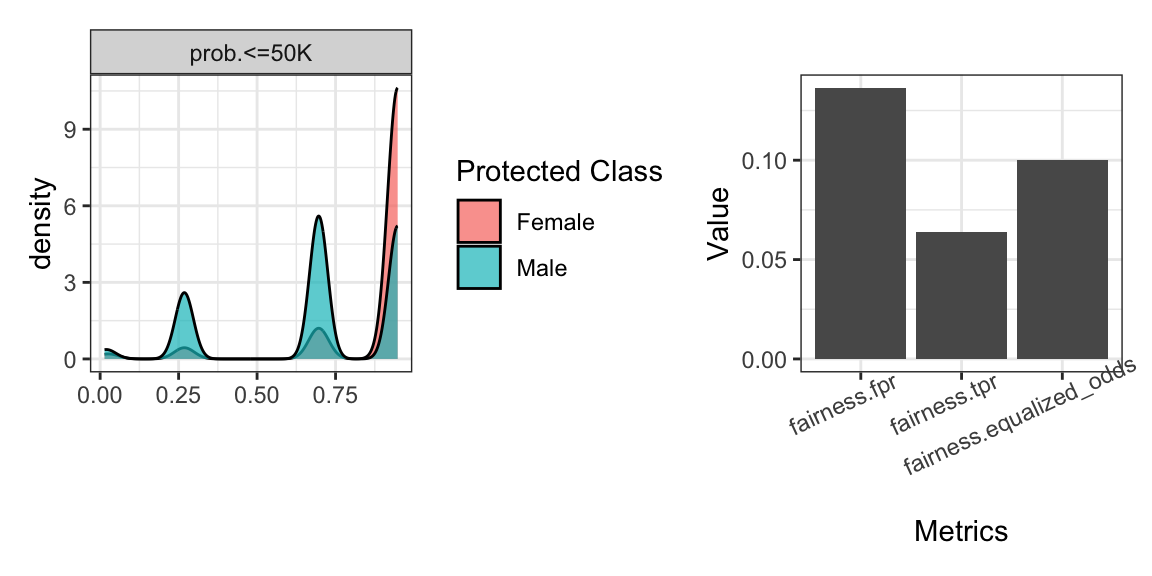
\includegraphics{RJ-2023-034_files/figure-latex/predplots-1} 

}

\caption{Visualizing predictions of the decision tree model. Left: Prediction densities for the negative class for Female and Male. Right: Fairness metrics comparison for FPR, TPR, EOd metrics. Plots show a higher likelihood for the '<50k' class for females resulting in fairness metrics different from 0.}\label{fig:predplots}
\end{figure}

\hypertarget{bias-mitigation-1}{%
\subsubsection{Bias mitigation}\label{bias-mitigation-1}}

As mentioned above, several ways to improve a model's fairness exist.
While non-technical interventions, such as e.g.~collecting more data should be preferred,
\CRANpkg{mlr3fairness} provides several bias mitigation techniques that can be used together with a \texttt{Learner} to obtain fairer models.
Table \ref{tab:biasmitigation} provides an overview of implemented bias mitigation techniques.
They are implemented as \texttt{PipeOps} from the \CRANpkg{mlr3pipelines} package and can be
combined with arbitrary learners using the \texttt{\%\textgreater{}\textgreater{}\%} operator to build a pipeline that can later be trained.
In the following example, we show how to combine a learner with a reweighing scheme (\texttt{reweighing\_wts}) or alternatively how to post-process predictions using the equalized odds debiasing (\texttt{EOd}) strategy.
An introduction to \CRANpkg{mlr3pipelines} is available in the corresponding \href{https://mlr3book.mlr-org.com/pipelines.html}{mlr3book chapter} (Bernd Bischl 2024).

\begin{verbatim}
po("reweighing_wts") %>>% lrn("classif.glmnet")
po("learner_cv", lrn("classif.glmnet")) %>>% po("EOd")
\end{verbatim}

\begin{longtable}[]{@{}
  >{\raggedright\arraybackslash}p{(\columnwidth - 6\tabcolsep) * \real{0.2065}}
  >{\raggedright\arraybackslash}p{(\columnwidth - 6\tabcolsep) * \real{0.3696}}
  >{\raggedright\arraybackslash}p{(\columnwidth - 6\tabcolsep) * \real{0.2065}}
  >{\raggedright\arraybackslash}p{(\columnwidth - 6\tabcolsep) * \real{0.2174}}@{}}
\caption{\label{tab:biasmitigation} Overview of bias mitigation techniques available in mlr3fairness.}\tabularnewline
\toprule\noalign{}
\begin{minipage}[b]{\linewidth}\raggedright
Key
\end{minipage} & \begin{minipage}[b]{\linewidth}\raggedright
Description
\end{minipage} & \begin{minipage}[b]{\linewidth}\raggedright
Type
\end{minipage} & \begin{minipage}[b]{\linewidth}\raggedright
Reference
\end{minipage} \\
\midrule\noalign{}
\endfirsthead
\toprule\noalign{}
\begin{minipage}[b]{\linewidth}\raggedright
Key
\end{minipage} & \begin{minipage}[b]{\linewidth}\raggedright
Description
\end{minipage} & \begin{minipage}[b]{\linewidth}\raggedright
Type
\end{minipage} & \begin{minipage}[b]{\linewidth}\raggedright
Reference
\end{minipage} \\
\midrule\noalign{}
\endhead
\bottomrule\noalign{}
\endlastfoot
EOd & Equalized-Odds Debiasing & Postprocessing & Hardt, Price, and Srebro (2016) \\
reweighing\_os & Reweighing (Oversampling) & Preprocessing & Kamiran and Calders (2012) \\
reweighing\_wts & Reweighing (Instance weights) & Preprocessing & Kamiran and Calders (2012) \\
\end{longtable}

It is simple for users or package developers to extend \CRANpkg{mlr3fairness} with additional
bias mitigation methods -- as an example, the \CRANpkg{mcboost} package adds further post-processing methods
that can improve fairness.
Along with pipeline operators, \CRANpkg{mlr3fairness} contains several machine learning algorithms listed in table \ref{tab:fairlearns} that can directly incorporate
fairness constraints. They can similarly be constructed using the \texttt{lrn()} shorthand.

\begin{longtable}[]{@{}lll@{}}
\caption{\label{tab:fairlearns} Overview of fair ML algorithms available with mlr3fairness.}\tabularnewline
\toprule\noalign{}
Key & Package & Reference \\
\midrule\noalign{}
\endfirsthead
\toprule\noalign{}
Key & Package & Reference \\
\midrule\noalign{}
\endhead
\bottomrule\noalign{}
\endlastfoot
regr.fairfrrm & fairml & Scutari, Panero, and Proissl (2021) \\
classif.fairfgrrm & fairml & Scutari, Panero, and Proissl (2021) \\
regr.fairzlm & fairml & Zafar et al. (2017) \\
classif.fairzlrm & fairml & Zafar et al. (2017) \\
regr.fairnclm & fairml & Komiyama et al. (2018) \\
\end{longtable}

\hypertarget{reports}{%
\subsubsection{Reports}\label{reports}}

Because fairness aspects can not always be investigated based on the fairness definitions above (e.g., due to biased sampling or labelling procedures), it is important to document data collection and the resulting data as well as the models resulting from this data.
Informing auditors about those aspects of a deployed model can lead to better assessments of a model's fairness.
Questionnaires for ML models (M. Mitchell et al. 2019) and data sets (Gebru et al. 2021) have been proposed in literature.
We further add automated report templates using R markdown (Xie, Dervieux, and Riederer 2020) for data sets and ML models.
In addition, we provide a template for a \emph{fairness report} which includes many fairness metrics and visualizations to provide a good starting point for generating a fairness report inspired by the \emph{Aequitas Toolkit} (Saleiro et al. 2018).
A preview for the different reports can be obtained from the \href{https://mlr3fairness.mlr-org.com/articles/reports-vignette.html}{Reports vignette} in the package documentation.

\begin{longtable}[]{@{}
  >{\raggedright\arraybackslash}p{(\columnwidth - 4\tabcolsep) * \real{0.2667}}
  >{\raggedright\arraybackslash}p{(\columnwidth - 4\tabcolsep) * \real{0.3467}}
  >{\raggedright\arraybackslash}p{(\columnwidth - 4\tabcolsep) * \real{0.3867}}@{}}
\caption{\label{tab:reports} Overview of reports generated by mlr3fairness.}\tabularnewline
\toprule\noalign{}
\begin{minipage}[b]{\linewidth}\raggedright
Report
\end{minipage} & \begin{minipage}[b]{\linewidth}\raggedright
Description
\end{minipage} & \begin{minipage}[b]{\linewidth}\raggedright
Reference
\end{minipage} \\
\midrule\noalign{}
\endfirsthead
\toprule\noalign{}
\begin{minipage}[b]{\linewidth}\raggedright
Report
\end{minipage} & \begin{minipage}[b]{\linewidth}\raggedright
Description
\end{minipage} & \begin{minipage}[b]{\linewidth}\raggedright
Reference
\end{minipage} \\
\midrule\noalign{}
\endhead
\bottomrule\noalign{}
\endlastfoot
\href{https://mlr3fairness.mlr-org.com/articles/modelcard/modelcard.html}{\texttt{report\_modelcard()}} & Modelcard for ML models & M. Mitchell et al. (2019) \\
\href{https://mlr3fairness.mlr-org.com/articles/datasheet/datasheet.html}{\texttt{report\_datasheet()}} & Datasheet for data sets & Gebru et al. (2021) \\
\href{https://mlr3fairness.mlr-org.com/articles/fairness/fairness.html}{\texttt{report\_fairness()}} & Fairness Report & -- \\
\end{longtable}

\hypertarget{case-study}{%
\section{Case study}\label{case-study}}

In order to demonstrate a full workflow, we conduct full bias assessment and bias mitigation on the popular adult data set (Dua and Graff 2017).
The goal is to predict whether an individual's income is larger than \$\(50.000\) with the sensitive attribute being \emph{gender}.
The data set is included with \CRANpkg{mlr3fairness}, separated into a \emph{train} and \emph{test} task and can be instantiated using \texttt{tsk("adult\_train")} and \texttt{tsk("adult\_test")}, respectively.
As a fairness metric, we consider \emph{true positive parity} which calls for equality in the true positive rates across groups, in this case the \texttt{sex} variable.
We furthermore are interested in the model's utility, here measured as its classification accuracy.

\begin{verbatim}
library("mlr3verse")
library("mlr3fairness")

task = tsk("adult_train")
print(task)
\end{verbatim}

\begin{verbatim}
#> <TaskClassif:adult_train> (30718 x 13)
#> * Target: target
#> * Properties: twoclass
#> * Features (12):
#>   - fct (7): education, marital_status, occupation, race, relationship,
#>     sex, workclass
#>   - int (5): age, capital_gain, capital_loss, education_num,
#>     hours_per_week
#> * Protected attribute: sex
\end{verbatim}

\begin{verbatim}
measures = msrs(c("fairness.tpr", "classif.acc"))
\end{verbatim}

In order to get an initial perspective, we benchmark three models using 3-fold cross-validation each:

\begin{itemize}
\tightlist
\item
  a classification tree from the \CRANpkg{rpart} package,
\item
  a penalized logistic regression from the \CRANpkg{glmnet} package and
\item
  a penalized logistic regression from the \CRANpkg{glmnet} package, but with reweighing pre-
  processing.
\end{itemize}

The logistic regression in the latter two approaches does not support operating on factor features natively, therefore we pre-process the data with a feature encoder from \CRANpkg{mlr3pipelines}.
To achieve this, we connect the feature encoder \texttt{po("encode")} with the learner using the \texttt{\%\textgreater{}\textgreater{}\%} operator.
This encodes factor variables into integers using dummy encoding.
We then evaluate all three learners on the \texttt{adult\_train} data using 3-fold cross-validation by building up a grid of experiments we want to run using \texttt{benchmark\_grid}.
This grid is then executed using the \texttt{benchmark} function, and we can aggregate the performance and fairness metric scores via the \texttt{\$aggregate()} function.

\begin{verbatim}
set.seed(4321)
learners = list(
    lrn("classif.rpart"),
    po("encode") %>>% lrn("classif.glmnet"),
    po("encode") %>>% po("reweighing_wts") %>>% lrn("classif.glmnet")
)

grid = benchmark_grid(
  tasks = tsks("adult_train"),
  learners = learners,
  resamplings = rsmp("cv", folds = 3)
)

bmr1 = benchmark(grid)
bmr1$aggregate(measures)[, c(4, 7, 8)]
\end{verbatim}

\begin{verbatim}
#>                              learner_id fairness.tpr classif.acc
#> 1:                        classif.rpart     0.059767      0.8408
#> 2:                encode.classif.glmnet     0.070781      0.8411
#> 3: encode.reweighing_wts.classif.glmnet     0.004732      0.8351
\end{verbatim}

The pre-processing step of reweighing already improved the fairness while sacrificing only a tiny bit of performance.
To see if we can further improve, we use \CRANpkg{mlr3tuning} to jointly tune all hyperparameters of the \emph{glmnet} model as well as our reweighing hyperparameter.
In order to do this, we use an \texttt{AutoTuner} from \CRANpkg{mlr3tuning}; a model that tunes its own hyperparameters during training.
The full code for setting up this model can be found in the appendix.
An \texttt{AutoTuner} requires a specific metric to tune for.
Here, we define a fairness-thresholded accuracy metric. We set \(\epsilon = 0.01\) as a threshold:

\[
  if \; |\Delta_{EOd}| \leq \epsilon: \textrm{accuracy} \;\; else: \;  - |\Delta_{EOd}|.
\]

\begin{verbatim}
metric = msr("fairness.constraint",
    performance_measure = msr("classif.acc"),
    fairness_measure = msr("fairness.eod"),
    epsilon = 0.01
)
\end{verbatim}

We then design the pipeline and the hyperparameters we want to tune over.
In the following example, we choose \texttt{tuning\_iters\ =\ 3} and set a small range for the hyperparameters in \texttt{vals} to shorten the run time of the tuning procedure.
In real settings, this parameter would be set to a larger number, such as \(100\).
To construct a self-tuning learner, we construct an \texttt{AutoTuner} that takes as input a learner, the resampling procedure and metric used for tuning as well as the tuning strategy along with a termination criterion (here how many tuning iterations should be run).
In addition, we provide a new \texttt{id} for the learner to beautify subsequent printing and visualization.
We can then use this self-tuning learner like any other learner and benchmark it using \texttt{benchmark} as described above.

\begin{verbatim}
tuning_iters = 3
at = AutoTuner$new(lrn, rsmp("holdout"),
    metric,
    tuner = mlr3tuning::tnr("random_search"),
    terminator = trm("evals", n_evals = tuning_iters)
)
at$id = "glmnet_weighted_tuned"

grd = benchmark_grid(
  tasks = tsks("adult_train"),
  learners = list(at),
  resamplings = rsmp("cv", folds = 3)
)

bmr2 = benchmark(grd, store_models = TRUE)
bmr2$aggregate(measures)[, c(4, 7, 8)]
\end{verbatim}

\begin{verbatim}
#>               learner_id fairness.tpr classif.acc
#> 1: glmnet_weighted_tuned     0.009486      0.8385
\end{verbatim}

The result improves w.r.t.~accuracy while only slightly decreasing the measured fairness.
Note that the generalization error is estimated using a holdout strategy during training and slight violations of the desired threshold \(\epsilon\) should therefore be considered (Feurer et al. 2023).
The results of both benchmark experiments can then be collected and jointly visualized in Figure \ref{fig:fat} visualizing accuracy and fairness of models in our benchmark.
In addition to aggregate scores (denoted by a cross) individual iterations of the 3-fold Cross-Validation (represented by points) are shown to visualize variations in the individual results.

\begin{figure}

{\centering 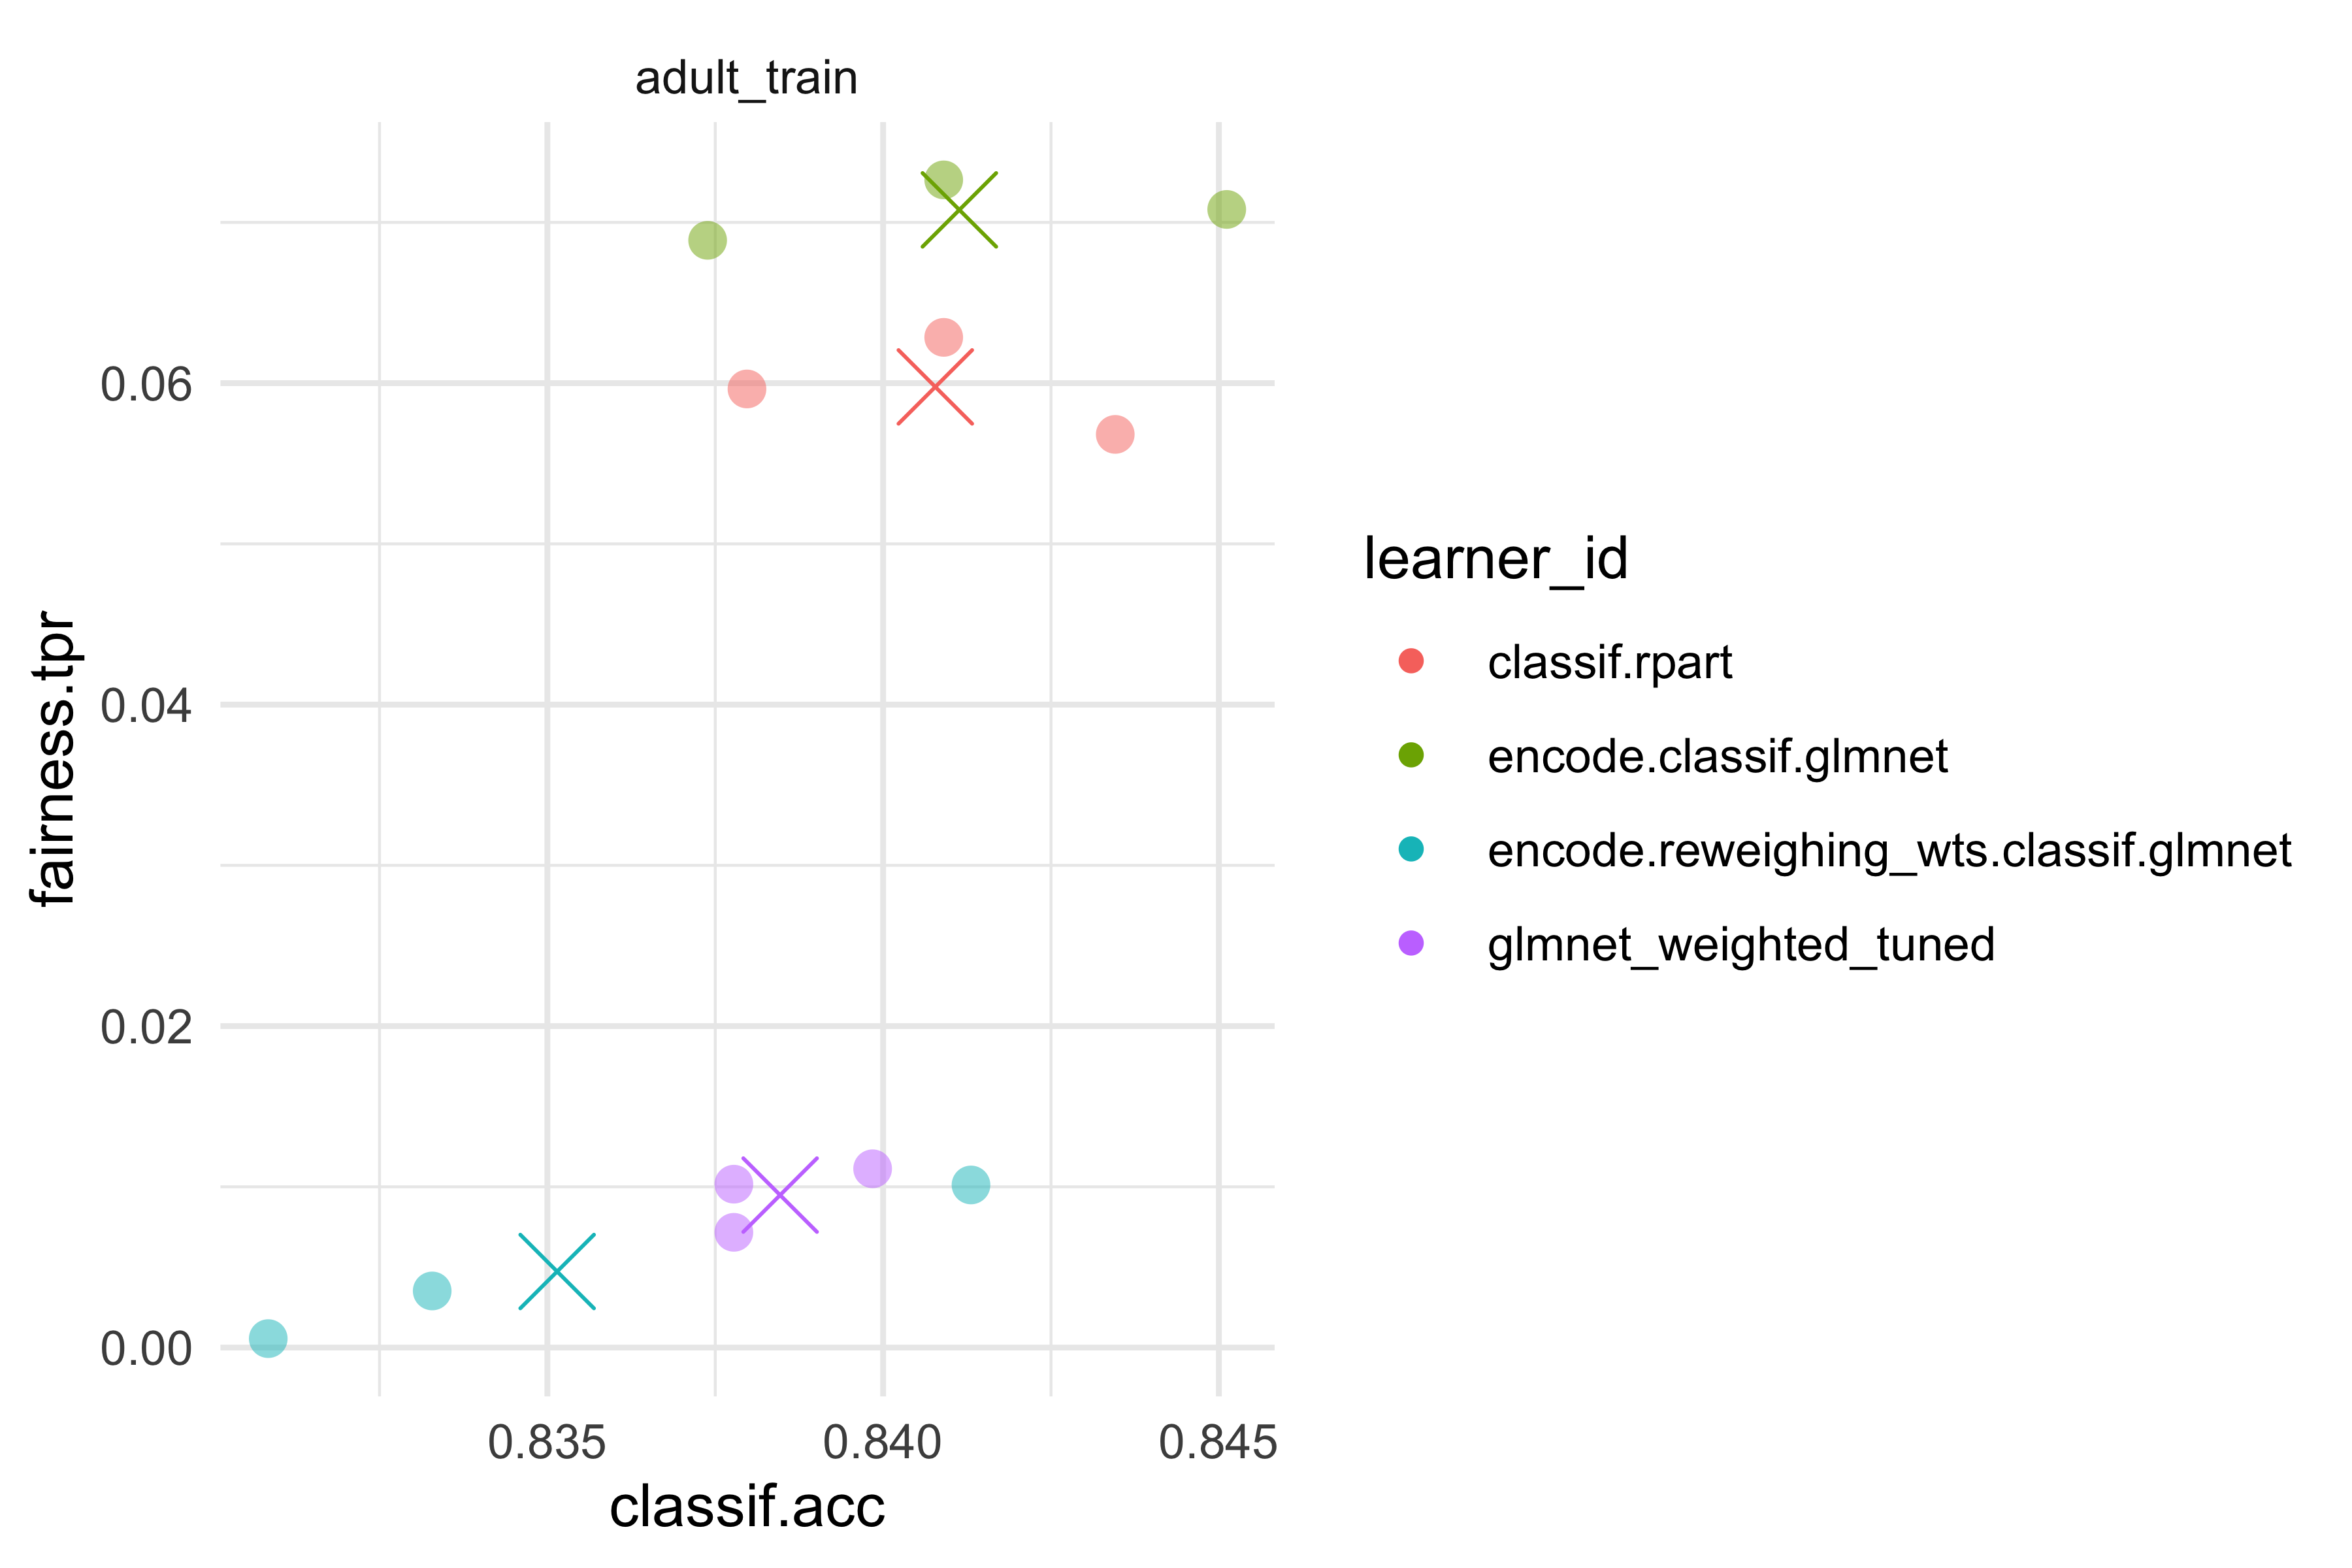
\includegraphics{RJ-2023-034_files/figure-latex/fat-1} 

}

\caption{Fairness-Accuracy tradeoff for 3-fold CV on the adult train set.}\label{fig:fat}
\end{figure}

\begin{verbatim}
bmr$aggregate(measures)[, c(4, 7, 8)]
\end{verbatim}

\begin{verbatim}
#>                              learner_id fairness.tpr classif.acc
#> 1:                        classif.rpart     0.059767      0.8408
#> 2:                encode.classif.glmnet     0.070781      0.8411
#> 3: encode.reweighing_wts.classif.glmnet     0.004732      0.8351
#> 4:                glmnet_weighted_tuned     0.009486      0.8385
\end{verbatim}

Especially when considering optimizing accuracy while still retaining a fair model, tuning can be helpful and further improve upon available trade-offs.
In this example, the \texttt{AutoTuner} improves w.r.t. the fairness metric while offering accuracy comparable with the simple \texttt{glmnet} model.
This can be observed from the fairness accuracy tradeoff shown in Figure \ref{fig:fat}.
Whether the achieved accuracy is sufficient needs to be determined, e.g.~from a business context.
For now, we assume that the model obtained from the \texttt{AutoTuner} is the model we might want to use going forward.
Having decided on a final model, we can now train the final model on the full training data

\begin{verbatim}
at_lrn = bmr$learners$learner[[4]]
at_lrn$train(tsk("adult_train"))
\end{verbatim}

and predict on the held out \emph{test} set available for the \texttt{Adult} dataset to obtain a final estimate.
This is important since estimating fairness metrics often incurs significant variance (Agrawal, Pfisterer, et al. 2020) and evaluation of the test-set provides us with an unbiased estimate of model performance after the previous model selection step.

\begin{verbatim}
test = tsk("adult_test")
at_lrn$predict(test)$score(measures, test)
\end{verbatim}

\begin{verbatim}
#> fairness.tpr  classif.acc 
#>      0.07141      0.84375
\end{verbatim}

On the held-out test set, the fairness constraint is slightly violated which can happen due to the comparatively large variance in the estimation of fairness metrics.

\hypertarget{summary}{%
\section{Summary}\label{summary}}

The large-scale availability and use of automated decision making systems have resulted in growing concerns for a lack of fairness in the decisions made by such systems.
As a result, fairness auditing methods, that allow for investigating (un-)fairness in such systems are an important step towards improving the auditability of deployed systems.
For ease of use, it is especially important, that they provide interoperability with machine learning toolkits that allows for ease of use and integration into model evaluation and tuning.
In future work we plan on implementing several tools that further support the user w.r.t. pinpointing potential fairness issues in the data, especially through the help of interpretability tools, such as the \CRANpkg{iml} (Molnar, Bischl, and Casalicchio 2018) package.
We furthermore aim to implement additional fairness metrics from the realm of `individual fairness' (Dwork et al. 2012) and `conditional demographic parity' (Wachter, Mittelstadt, and Russell 2020).

\pagebreak

\hypertarget{appendix}{%
\section{Appendix}\label{appendix}}

\hypertarget{tuning-the-ml-pipeline}{%
\subsection{Tuning the ML pipeline}\label{tuning-the-ml-pipeline}}

We include the full code to construct the \texttt{AutoTuner} with additional details
and comments below.
We first load all required packages and use \pkg{mlr3}'s interaction with the \CRANpkg{future} (Bengtsson 2021) package
to automatically distribute the tuning to all available cores in parallel by setting a \texttt{plan}.
See the documentation of \CRANpkg{future} for platform-specific hints regarding parallelization.

\begin{verbatim}
library(mlr3misc)
library(mlr3)
library(mlr3pipelines)
library(mlr3fairness)
library(mlr3tuning)

# Enable parallelization utilizing all cores
future::plan("multicore")
\end{verbatim}

We then instantiate an ML pipeline using \pkg{mlr3pipelines}.
This connects several modelling steps, in our case \textbf{categorical encoding}, \textbf{reweighing} and a final \textbf{learner} using the
\texttt{\%\textgreater{}\textgreater{}\%} (double caret) operator, ultimately forming a new learner.
This learner can then subsequently be fit on a \texttt{Task}. We use the \texttt{po(\textless{}key\textgreater{})} shorthand to construct a new
pipeline operator from a dictionary of implemented operators.
We conduct \textbf{categorical encoding} because \pkg{glmnet} can not naturally handle categorical variables, and we therefore have
to encode them (in our case using \texttt{one-hot} encoding).

\begin{verbatim}
# Define the learner pipeline.
lrn = as_learner(po("encode") %>>% po("reweighing_wts") %>>%
  po("learner", lrn("classif.glmnet")))
\end{verbatim}

In addition, we have to specify the hyperparameter space our \texttt{Tuner} should tune over.
We do this by defining a list of values with a \texttt{to\_tune()} token specifying the range.
Note, that hyperparameter names are prefixed with the respective operation's \texttt{id}.

\begin{verbatim}
# Define the parameter space to optimize over
vals = list(
  reweighing_wts.alpha = to_tune(0.75, 1),
  classif.glmnet.alpha = to_tune(0.5, 1),
  classif.glmnet.s = to_tune(1e-4, 1e-2, logscale = TRUE)
)

# Add search space to the learner
lrn$param_set$values = insert_named(lrn$param_set$values, vals)
\end{verbatim}

Before we now train the model, we again specify a metric we aim to satisfy, here we would like the equalized odds difference to be smaller than \(0.1\).
In this case, we set a constraint on the \emph{equalized odds difference} comprised of the differences in true positive rate (TPR) and false positive rate (FPR):

\[
\Delta_{EOd} = \frac{|\textrm{TPR}_{sex = M} - \textrm{TPR}_{sex = F}| + |\textrm{FPR}_{sex = M} - \textrm{FPR}_{sex = F}|}{2}.
\]

This can be done using the \texttt{fairness.constraint} measure.

\begin{verbatim}
metric = msr("fairness.constraint",
    performance_measure = msr("classif.acc"),
    fairness_measure = msr("fairness.eod"),
    epsilon = 0.1
)
\end{verbatim}

We can now instantiate a new \texttt{AutoTuner} using \texttt{lrn} defined above by additionally providing arguments specifying the tuning strategy, in our case random search, the measure to optimize for as well as the number of tuning steps.

\begin{verbatim}
metric = msr("fairness.constraint",
    performance_measure = msr("classif.acc"),
    fairness_measure = msr("fairness.eod"),
    epsilon = 0.1
)

at = AutoTuner$new(
  learner = lrn, # The learner
  resampling = rsmp("holdout"), # inner resampling strategy
  measure = metric, # the metric to optimize for
  tuner = mlr3tuning::tnr("random_search"), # tuning strategy
  terminator = trm("evals", n_evals = 30) # number of tuning steps
)
\end{verbatim}

The so-constructed \texttt{AutoTuner} can now be used on any classification Task!
Additional information regarding the \texttt{AutoTuner} is again available in the corresponding \href{https://mlr3book.mlr-org.com/optimization.html\#autotuner}{mlr3book chapter}.
In the following example, we will apply it to the \texttt{Adult} task and train our model.
This will perform a tuning loop for the specified number of evaluations and
automatically retrain the best found parameters on the full data.

\begin{verbatim}
at$train(tsk("adult_train"))
\end{verbatim}

After training, we can look at the best models found, here ordered by our metric.
Note, that our metric reports the negative constraint violation if the constraint is violated and the accuracy in case the constraint is satisfied.

\begin{verbatim}
head(at$archive$data[order(fairness.acc_equalized_odds_cstrt), 1:4])
\end{verbatim}

\begin{verbatim}
#>    reweighing_wts.alpha classif.glmnet.alpha classif.glmnet.s
#> 1:               0.9503               0.5138           -4.654
#> 2:               0.8160               0.9289           -5.314
#> 3:               0.7507               0.6784           -5.786
#> 4:               0.9694               0.9219           -6.198
#> 5:               0.8254               0.8826           -7.241
#> 6:               0.8808               0.7362           -7.311
#>    fairness.acc_equalized_odds_cstrt
#> 1:                            0.8411
#> 2:                            0.8445
#> 3:                            0.8447
#> 4:                            0.8448
#> 5:                            0.8448
#> 6:                            0.8448
\end{verbatim}

We can then use the tuned model to assess our metric on the held out data:

\begin{verbatim}
prd = at$predict(tsk("adult_test"))
prd$score(c(metric, msr("classif.acc"), msr("fairness.eod")),  tsk("adult_test"))
\end{verbatim}

\begin{verbatim}
#> fairness.acc_equalized_odds_cstrt                       classif.acc 
#>                           0.83976                           0.83976 
#>           fairness.equalized_odds 
#>                           0.07512
\end{verbatim}

So our tuned model manages to obtain an accuracy of \texttt{\textasciitilde{}0.84} while satisfying the specified constraint of \(\Delta_{EOd} < 0.1\).
So to summarize, we have tuned a model to optimize accuracy with respect to a constraint on a selected fairness metric using an \texttt{AutoTuner}.

\hypertarget{references}{%
\section*{References}\label{references}}
\addcontentsline{toc}{section}{References}

\hypertarget{refs}{}
\begin{CSLReferences}{1}{0}
\leavevmode\vadjust pre{\hypertarget{ref-fairnessjl}{}}%
Agrawal, Ashrya, Jiahao Chen, Sebastian Vollmer, and Anthony Blaom. 2020. {``Fairness.jl.''} Zenodo. \url{https://doi.org/10.5281/zenodo.3977197}.

\leavevmode\vadjust pre{\hypertarget{ref-agrawal2020debiasing}{}}%
Agrawal, Ashrya, Florian Pfisterer, Bernd Bischl, Jiahao Chen, Srijan Sood, Sameena Shah, Francois Buet-Golfouse, Bilal A Mateen, and Sebastian Vollmer. 2020. {``Debiasing Classifiers: Is Reality at Variance with Expectation?''} \emph{arXiv:2011.02407}.

\leavevmode\vadjust pre{\hypertarget{ref-fairwashing}{}}%
Aivodji, Ulrich, Hiromi Arai, Olivier Fortineau, Sébastien Gambs, Satoshi Hara, and Alain Tapp. 2019. {``Fairwashing: The Risk of Rationalization.''} In \emph{International Conference on Machine Learning}, 97:161--70. PMLR.

\leavevmode\vadjust pre{\hypertarget{ref-compas}{}}%
Angwin, Julia, Jeff Larson, Surya Mattu, and Lauren Kichner. 2016. {``Machine Bias.''} ProPublica. \url{https://www.propublica.org/article/machine-bias-risk-assessments-in-criminal-sentencing}.

\leavevmode\vadjust pre{\hypertarget{ref-bao2021s}{}}%
Bao, Michelle, Angela Zhou, Samantha A Zottola, Brian Brubach, Sarah Desmarais, Aaron Seth Horowitz, Kristian Lum, and Suresh Venkatasubramanian. 2021. {``It's COMPASlicated: The Messy Relationship Between RAI Datasets and Algorithmic Fairness Benchmarks.''} In \emph{Thirty-Fifth Conference on Neural Information Processing Systems Datasets and Benchmarks Track (Round 1)}.

\leavevmode\vadjust pre{\hypertarget{ref-fairmlbook}{}}%
Barocas, Solon, Moritz Hardt, and Arvind Narayanan. 2019. \emph{Fairness and Machine Learning}. fairmlbook.org. \url{https://fairmlbook.org/}.

\leavevmode\vadjust pre{\hypertarget{ref-mlr3tuning}{}}%
Becker, Marc, Michel Lang, Jakob Richter, Bernd Bischl, and Daniel Schalk. 2023. \emph{Mlr3tuning: Hyperparameter Optimization for 'Mlr3'}.

\leavevmode\vadjust pre{\hypertarget{ref-bbotk}{}}%
Becker, Marc, Jakob Richter, Michel Lang, Bernd Bischl, and Martin Binder. 2023. \emph{Bbotk: Black-Box Optimization Toolkit}.

\leavevmode\vadjust pre{\hypertarget{ref-aif360}{}}%
Bellamy, Rachel KE, Kuntal Dey, Michael Hind, Samuel C Hoffman, Stephanie Houde, Kalapriya Kannan, Pranay Lohia, et al. 2019. {``{AI Fairness 360}: An Extensible Toolkit for Detecting and Mitigating Algorithmic Bias.''} \emph{IBM Journal of Research and Development} 63 (4/5): 4--1. \url{https://aif360.mybluemix.net/}.

\leavevmode\vadjust pre{\hypertarget{ref-future}{}}%
Bengtsson, Henrik. 2021. {``A Unifying Framework for Parallel and Distributed Processing in {R} Using Futures.''} \emph{The R Journal} 13 (2): 208--27. \url{https://doi.org/10.32614/RJ-2021-048}.

\leavevmode\vadjust pre{\hypertarget{ref-richardcompas}{}}%
Berk, Richard, Hoda Heidari, Shahin Jabbari, Michael Kearns, and Aaron Roth. 2018. {``{Fairness in Criminal Justice Risk Assessments: The State of the Art}.''} \emph{Sociological Methods \& Research}, August. \url{https://doi.org/10.1177/0049124118782533}.

\leavevmode\vadjust pre{\hypertarget{ref-mlr3book}{}}%
Bernd Bischl, Lars Kotthoff, Raphael Sonabend, ed. 2024. \emph{Applied Machine Learning Using Mlr3 in {R}}. CRC Press. \url{https://mlr3book.mlr-org.com}.

\leavevmode\vadjust pre{\hypertarget{ref-dalex}{}}%
Biecek, Przemyslaw. 2018. {``{DALEX}: {Explainers for Complex Predictive Models} in {R}.''} \emph{Journal of Machine Learning Research} 19 (84): 1--5. \url{https://jmlr.org/papers/v19/18-416.html}.

\leavevmode\vadjust pre{\hypertarget{ref-mlr3pipelines}{}}%
Binder, Martin, Florian Pfisterer, Michel Lang, Lennart Schneider, Lars Kotthoff, and Bernd Bischl. 2021. {``{mlr3pipelines - Flexible Machine Learning Pipelines in R}.''} \emph{Journal of Machine Learning Research} 22 (184): 1--7. \url{https://jmlr.org/papers/v22/21-0281.html}.

\leavevmode\vadjust pre{\hypertarget{ref-binns2020apparent}{}}%
Binns, Reuben. 2020. {``On the Apparent Conflict Between Individual and Group Fairness.''} In \emph{Proceedings of the Conference on Fairness, Accountability, and Transparency}, 514--24. New York, NY, USA: Association for Computing Machinery. \url{https://doi.org/10.1145/3351095.3372864}.

\leavevmode\vadjust pre{\hypertarget{ref-fairlearn}{}}%
Bird, Sarah, Miro Dudík, Richard Edgar, Brandon Horn, Roman Lutz, Vanessa Milan, Mehrnoosh Sameki, Hanna Wallach, and Kathleen Walker. 2020. {``Fairlearn: A Toolkit for Assessing and Improving Fairness in {AI}.''} MSR-TR-2020-32. Microsoft. \url{https://www.microsoft.com/en-us/research/publication/fairlearn-a-toolkit-for-assessing-and-improving-fairness-in-ai/}.

\leavevmode\vadjust pre{\hypertarget{ref-mlr}{}}%
Bischl, Bernd, Michel Lang, Lars Kotthoff, Julia Schiffner, Jakob Richter, Erich Studerus, Giuseppe Casalicchio, and Zachary M. Jones. 2016. {``{mlr}: Machine Learning in {R}.''} \emph{Journal of Machine Learning Research} 17 (170): 1--5. \url{https://jmlr.org/papers/v17/15-066.html}.

\leavevmode\vadjust pre{\hypertarget{ref-bischl2012resampling}{}}%
Bischl, Bernd, Olaf Mersmann, Heike Trautmann, and Claus Weihs. 2012. {``Resampling Methods for Meta-Model Validation with Recommendations for Evolutionary Computation.''} \emph{Evolutionary Computation} 20 (2): 249--75.

\leavevmode\vadjust pre{\hypertarget{ref-gendershades}{}}%
Buolamwini, Joy, and Timnit Gebru. 2018. {``{Gender shades: Intersectional accuracy disparities in commercial gender classification}.''} In \emph{Proceedings of the Conference on Fairness, Accountability, and Transparency}, 77--91. PMLR.

\leavevmode\vadjust pre{\hypertarget{ref-Calders2010}{}}%
Calders, Toon, and Sicco Verwer. 2010. {``{Three naive Bayes approaches for discrimination-free classification}.''} \emph{Data Mining and Knowledge Discovery} 21 (2): 277--92. \url{https://doi.org/10.1007/s10618-010-0190-x}.

\leavevmode\vadjust pre{\hypertarget{ref-Chen2018}{}}%
Chen, Jiahao. 2018. {``Fair Lending Needs Explainable Models for Responsible Recommendation.''} In \emph{Proceedings of the 2nd FATREC Workshop on Responsible Recommendation}.

\leavevmode\vadjust pre{\hypertarget{ref-chouldechova2017fair}{}}%
Chouldechova, Alexandra. 2017. {``Fair Prediction with Disparate Impact: A Study of Bias in Recidivism Prediction Instruments.''} \emph{Big Data} 5 (2): 153--63. \url{https://doi.org/10.1089/big.2016.0047}.

\leavevmode\vadjust pre{\hypertarget{ref-cirillo2020sex}{}}%
Cirillo, Davide, Silvina Catuara-Solarz, Czuee Morey, Emre Guney, Laia Subirats, Simona Mellino, Annalisa Gigante, et al. 2020. {``Sex and Gender Differences and Biases in Artificial Intelligence for Biomedicine and Healthcare.''} \emph{NPJ Digital Medicine} 3 (1): 1--11. \url{https://doi.org/10.1038/s41746-020-0288-5}.

\leavevmode\vadjust pre{\hypertarget{ref-corbett2018measure}{}}%
Corbett-Davies, Sam, and Sharad Goel. 2018. {``The Measure and Mismeasure of Fairness: A Critical Review of Fair Machine Learning.''} \emph{arXiv:1808.00023}.

\leavevmode\vadjust pre{\hypertarget{ref-corbettcompas}{}}%
Corbett-Davies, Sam, Emma Pierson, Avi Feller, Sharad Goel, and Aziz Huq. 2017. {``Algorithmic Decision Making and the Cost of Fairness.''} In \emph{Proceedings of the 23rd ACM SIGKDD International Conference on Knowledge Discovery and Data Mining}, 797--806. KDD '17. New York, NY, USA: Association for Computing Machinery. \url{https://doi.org/10.1145/3097983.3098095}.

\leavevmode\vadjust pre{\hypertarget{ref-dawes1989clinical}{}}%
Dawes, Robyn M, David Faust, and Paul E Meehl. 1989. {``Clinical Versus Actuarial Judgment.''} \emph{Science} 243 (4899): 1668--74. \url{https://doi.org/10.1126/science.2648573}.

\leavevmode\vadjust pre{\hypertarget{ref-uci}{}}%
Dua, Dheeru, and Casey Graff. 2017. {``{UCI} Machine Learning Repository.''} University of California, Irvine, School of Information; Computer Sciences. \url{http://archive.ics.uci.edu/ml}.

\leavevmode\vadjust pre{\hypertarget{ref-dwork2012}{}}%
Dwork, Cynthia, Moritz Hardt, Toniann Pitassi, Omer Reingold, and Richard Zemel. 2012. {``Fairness Through Awareness.''} In \emph{Proceedings of the 3rd Innovations in Theoretical Computer Science Conference}, 214--26.

\leavevmode\vadjust pre{\hypertarget{ref-eubanks2018automating}{}}%
Eubanks, Virginia. 2018. \emph{Automating Inequality: How High-Tech Tools Profile, Police, and Punish the Poor}. St. Martin's Press.

\leavevmode\vadjust pre{\hypertarget{ref-feurer23}{}}%
Feurer, Matthias, Katharina Eggensperger, Edward Bergman, Florian Pfisterer, Bernd Bischl, and Frank Hutter. 2023. {``Mind the Gap: Measuring Generalization Performance Across Multiple Objectives.''} In \emph{Advances in Intelligent Data Analysis XXI}, 130--42.

\leavevmode\vadjust pre{\hypertarget{ref-friedler16}{}}%
Friedler, Sorelle A., Carlos Scheidegger, and Suresh Venkatasubramanian. 2016. {``On the (Im)possibility of Fairness.''} \emph{arXiv:1609.07236}.

\leavevmode\vadjust pre{\hypertarget{ref-galindo2000credit}{}}%
Galindo, Jorge, and Pablo Tamayo. 2000. {``Credit Risk Assessment Using Statistical and Machine Learning: Basic Methodology and Risk Modeling Applications.''} \emph{Computational Economics} 15 (1): 107--43.

\leavevmode\vadjust pre{\hypertarget{ref-datasheets}{}}%
Gebru, Timnit, Jamie Morgenstern, Briana Vecchione, Jennifer Wortman Vaughan, Hanna Wallach, Hal Daumé Iii, and Kate Crawford. 2021. {``Datasheets for Datasets.''} \emph{Communications of the ACM} 64 (12): 86--92.

\leavevmode\vadjust pre{\hypertarget{ref-hardt2016equality}{}}%
Hardt, Moritz, Eric Price, and Nati Srebro. 2016. {``Equality of Opportunity in Supervised Learning.''} \emph{Advances in Neural Information Processing Systems} 29: 3315--23.

\leavevmode\vadjust pre{\hypertarget{ref-kamiran2012data}{}}%
Kamiran, Faisal, and Toon Calders. 2012. {``Data Preprocessing Techniques for Classification Without Discrimination.''} \emph{Knowledge and Information Systems} 33 (1): 1--33.

\leavevmode\vadjust pre{\hypertarget{ref-kilbertus2017avoiding}{}}%
Kilbertus, Niki, Mateo Rojas Carulla, Giambattista Parascandolo, Moritz Hardt, Dominik Janzing, and Bernhard Schölkopf. 2017. {``Avoiding Discrimination Through Causal Reasoning.''} \emph{Advances in Neural Information Processing Systems} 30.

\leavevmode\vadjust pre{\hypertarget{ref-kim2020fact}{}}%
Kim, Joon Sik, Jiahao Chen, and Ameet Talwalkar. 2020. {``Fact: A Diagnostic for Group Fairness Trade-Offs.''} In \emph{International Conference on Machine Learning}, 5264--74. PMLR.

\leavevmode\vadjust pre{\hypertarget{ref-komiyama}{}}%
Komiyama, Junpei, Akiko Takeda, Junya Honda, and Hajime Shimao. 2018. {``Nonconvex Optimization for Regression with Fairness Constraints.''} In \emph{International Conference on Machine Learning}, 2737--46. PMLR.

\leavevmode\vadjust pre{\hypertarget{ref-kozodoi2022fairness}{}}%
Kozodoi, Nikita, Johannes Jacob, and Stefan Lessmann. 2022. {``Fairness in Credit Scoring: Assessment, Implementation and Profit Implications.''} \emph{European Journal of Operational Research} 297 (3): 1083--94. \url{https://doi.org/10.1016/j.ejor.2021.06.023}.

\leavevmode\vadjust pre{\hypertarget{ref-fairness}{}}%
Kozodoi, Nikita, and Tibor V. Varga. 2021. \emph{Fairness: Algorithmic Fairness Metrics}. \url{https://CRAN.R-project.org/package=fairness}.

\leavevmode\vadjust pre{\hypertarget{ref-caret}{}}%
Kuhn, Max. 2021. \emph{Caret: Classification and Regression Training}. \url{https://CRAN.R-project.org/package=caret}.

\leavevmode\vadjust pre{\hypertarget{ref-tidymodels}{}}%
Kuhn, Max, and Hadley Wickham. 2020. \emph{Tidymodels: A Collection of Packages for Modeling and Machine Learning Using Tidyverse Principles.} \url{https://www.tidymodels.org}.

\leavevmode\vadjust pre{\hypertarget{ref-mlr3}{}}%
Lang, Michel, Martin Binder, Jakob Richter, Patrick Schratz, Florian Pfisterer, Stefan Coors, Quay Au, Giuseppe Casalicchio, Lars Kotthoff, and Bernd Bischl. 2019. {``{mlr3}: A Modern Object-Oriented Machine Learning Framework in {R}.''} \emph{Journal of Open Source Software}, December. \url{https://doi.org/10.21105/joss.01903}.

\leavevmode\vadjust pre{\hypertarget{ref-mlr3verse}{}}%
Lang, Michel, and Patrick Schratz. 2023. \emph{Mlr3verse: Easily Install and Load the 'Mlr3' Package Family}.

\leavevmode\vadjust pre{\hypertarget{ref-mehrabi}{}}%
Mehrabi, Ninareh, Fred Morstatter, Nripsuta Saxena, Kristina Lerman, and Aram Galstyan. 2021. {``A Survey on Bias and Fairness in Machine Learning.''} \emph{ACM Computing Surveys (CSUR)} 54 (6): 1--35.

\leavevmode\vadjust pre{\hypertarget{ref-modelcards}{}}%
Mitchell, Margaret, Simone Wu, Andrew Zaldivar, Parker Barnes, Lucy Vasserman, Ben Hutchinson, Elena Spitzer, Inioluwa Deborah Raji, and Timnit Gebru. 2019. {``Model Cards for Model Reporting.''} In \emph{Proceedings of the Conference on Fairness, Accountability, and Transparency}, 220--29. New York, NY, USA: PMLR; Association for Computing Machinery. \url{https://doi.org/10.1145/3287560.3287596}.

\leavevmode\vadjust pre{\hypertarget{ref-mitchell2021algorithmic}{}}%
Mitchell, Shira, Eric Potash, Solon Barocas, Alexander D'Amour, and Kristian Lum. 2021. {``{Algorithmic fairness: Choices, assumptions, and definitions}.''} \emph{Annual Review of Statistics and Its Application} 8: 141--63. \url{https://doi.org/10.1146/annurev-statistics-042720-125902}.

\leavevmode\vadjust pre{\hypertarget{ref-iml}{}}%
Molnar, Christoph, Bernd Bischl, and Giuseppe Casalicchio. 2018. {``{iml}: An {R} Package for Interpretable Machine Learning.''} \emph{JOSS} 3 (26): 786. \url{https://doi.org/10.21105/joss.00786}.

\leavevmode\vadjust pre{\hypertarget{ref-noble2018algorithms}{}}%
Noble, Safiya Umoja. 2018. \emph{Algorithms of Oppression}. New York University Press.

\leavevmode\vadjust pre{\hypertarget{ref-o2016weapons}{}}%
O'neil, Cathy. 2016. \emph{Weapons of Math Destruction: How Big Data Increases Inequality and Threatens Democracy}. Crown.

\leavevmode\vadjust pre{\hypertarget{ref-sklearn}{}}%
Pedregosa, Fabian, Gaël Varoquaux, Alexandre Gramfort, Vincent Michel, Bertrand Thirion, Olivier Grisel, Mathieu Blondel, et al. 2011. {``Scikit-Learn: Machine Learning in Python.''} \emph{Journal of Machine Learning Research} 12: 2825--30.

\leavevmode\vadjust pre{\hypertarget{ref-perrone2021fair}{}}%
Perrone, Valerio, Michele Donini, Muhammad Bilal Zafar, Robin Schmucker, Krishnaram Kenthapadi, and Cédric Archambeau. 2021. {``{Fair Bayesian Optimization}.''} In \emph{Proceedings of the 2021 AAAI/ACM Conference on AI, Ethics, and Society}, 854--63.

\leavevmode\vadjust pre{\hypertarget{ref-mcboost}{}}%
Pfisterer, Florian, Christoph Kern, Susanne Dandl, Matthew Sun, Michael P. Kim, and Bernd Bischl. 2021. {``Mcboost: Multi-Calibration Boosting for {R}.''} \emph{Journal of Open Source Software} 6 (64): 3453. \url{https://doi.org/10.21105/joss.03453}.

\leavevmode\vadjust pre{\hypertarget{ref-superlearner}{}}%
Polley, Eric, Erin LeDell, Chris Kennedy, and Mark van der Laan. 2021. \emph{SuperLearner: Super Learner Prediction}. \url{https://CRAN.R-project.org/package=SuperLearner}.

\leavevmode\vadjust pre{\hypertarget{ref-R}{}}%
R Core Team. 2021. \emph{R: A Language and Environment for Statistical Computing}. Vienna, Austria: R Foundation for Statistical Computing. \url{http://www.R-project.org/}.

\leavevmode\vadjust pre{\hypertarget{ref-saleiro2018aequitas}{}}%
Saleiro, Pedro, Benedict Kuester, Loren Hinkson, Jesse London, Abby Stevens, Ari Anisfeld, Kit T Rodolfa, and Rayid Ghani. 2018. {``Aequitas: A Bias and Fairness Audit Toolkit.''} \emph{arXiv:1811.05577}.

\leavevmode\vadjust pre{\hypertarget{ref-schumann}{}}%
Schumann, Candice, Jeffrey S. Foster, Nicholas Mattei, and John P. Dickerson. 2020. {``We Need Fairness and Explainability in Algorithmic Hiring.''} In \emph{Proceedings of the 19th International Conference on Autonomous Agents and MultiAgent Systems}, 1716--20. AAMAS '20. Auckland, New Zealand: International Foundation for Autonomous Agents; Multiagent Systems.

\leavevmode\vadjust pre{\hypertarget{ref-schwobel-facct22a}{}}%
Schwöbel, P., and P. Remmers. 2022. {``The Long Arc of Fairness: Formalisations and Ethical Discourse.''} In \emph{Proceedings of the Conference on Fairness, Accountability, and Transparency}, 2179--88. New York, NY, USA: Association for Computing Machinery. \url{https://doi.org/10.1145/3531146.3534635}.

\leavevmode\vadjust pre{\hypertarget{ref-scutari}{}}%
Scutari, Marco, Francesca Panero, and Manuel Proissl. 2021. {``Achieving Fairness with a Simple Ridge Penalty.''} \emph{arXiv:2105.13817}.

\leavevmode\vadjust pre{\hypertarget{ref-mlr3proba}{}}%
Sonabend, Raphael, Franz J Király, Andreas Bender, Bernd Bischl, and Michel Lang. 2021. {``{mlr3proba: An {R} Package for Machine Learning in Survival Analysis}.''} \emph{Bioinformatics}, February. \url{https://doi.org/10.1093/bioinformatics/btab039}.

\leavevmode\vadjust pre{\hypertarget{ref-Topol2019}{}}%
Topol, Eric J. 2019. {``High-Performance Medicine: The Convergence of Human and Artificial Intelligence.''} \emph{Nature Medicine} 25 (1): 44--56. \url{https://doi.org/10.1038/s41591-018-0300-7}.

\leavevmode\vadjust pre{\hypertarget{ref-Turner2019}{}}%
Turner, Matthew, and Michael McBurnett. 2019. {``Predictive Models with Explanatory Concepts: A General Framework for Explaining Machine Learning Credit Risk Models That Simultaneously Increases Predictive Power.''} In \emph{Proceedings of the 15th Credit Scoring and Credit Control Conference}. \url{https://crc.business-school.ed.ac.uk/wp-content/uploads/sites/55/2019/07/C12-Predictive-Models-with-Explanatory-Concepts-McBurnett.pdf}.

\leavevmode\vadjust pre{\hypertarget{ref-Vanschoren2014}{}}%
Vanschoren, Joaquin, Jan N. van Rijn, Bernd Bischl, and Luis Torgo. 2014. {``{OpenML}.''} \emph{{ACM} {SIGKDD} Explorations Newsletter} 15 (2): 49--60. \url{https://doi.org/10.1145/2641190.2641198}.

\leavevmode\vadjust pre{\hypertarget{ref-wachter-vlr2020}{}}%
Wachter, S., B. Mittelstadt, and C. Russell. 2020. {``Bias Preservation in Machine Learning: The Legality of Fairness Metrics Under {EU} Non-Discrimination Law.''} \emph{West Virginia Law Review} 123.

\leavevmode\vadjust pre{\hypertarget{ref-chen22}{}}%
Watkins, Elizabeth Anne, Michael McKenna, and Jiahao Chen. 2022. {``The Four-Fifths Rule Is Not Disparate Impact: A Woeful Tale of Epistemic Trespassing in Algorithmic Fairness.''} \emph{arXiv:2202.09519}.

\leavevmode\vadjust pre{\hypertarget{ref-ggplot2}{}}%
Wickham, Hadley. 2016. \emph{Ggplot2: Elegant Graphics for Data Analysis}. Springer-Verlag New York. \url{https://ggplot2.tidyverse.org}.

\leavevmode\vadjust pre{\hypertarget{ref-fairmodels}{}}%
Wiśniewski, Jakub, and Przemysław Biecek. 2022. {``Fairmodels: A Flexible Tool for Bias Detection, Visualization, and Mitigation in Binary Classification Models.''} \emph{The R Journal} 14: 227--43. \url{https://rj.urbanek.nz/articles/RJ-2022-019/}.

\leavevmode\vadjust pre{\hypertarget{ref-rmarkdown}{}}%
Xie, Yihui, Christophe Dervieux, and Emily Riederer. 2020. \emph{R Markdown Cookbook}. Boca Raton, Florida: Chapman; Hall/CRC. \url{https://bookdown.org/yihui/rmarkdown-cookbook}.

\leavevmode\vadjust pre{\hypertarget{ref-Zafar2017}{}}%
Zafar, Muhammad Bilal, Isabel Valera, Manuel Gomez Rodriguez, and Krishna P. Gummadi. 2017. {``{Fairness beyond Disparate treatment {\&} Disparate Impact}.''} In \emph{Proceedings of the 26th International Conference on World Wide Web}, 1171--80. Geneva, Switzerland: International World Wide Web Conferences Steering Committee. \url{https://doi.org/10.1145/3038912.3052660}.

\end{CSLReferences}

\bibliography{mlr3fairness.bib}

\address{%
Florian Pfisterer\\
Ludwig-Maximilians-Universität München\\%
Munich, Germany\\
Munich Center for Machine Learning\\%
Munich, Germany\\
%
%
\textit{ORCiD: \href{https://orcid.org/0000-0001-8867-762X}{0000-0001-8867-762X}}\\%
\href{mailto:florian.pfisterer@stat.uni-muenchen.de}{\nolinkurl{florian.pfisterer@stat.uni-muenchen.de}}%
}

\address{%
Siyi Wei\\
University of Toronto\\%
Toronto, Canada\\
%
%
%
\href{mailto:weisiyi2@gmail.com}{\nolinkurl{weisiyi2@gmail.com}}%
}

\address{%
Sebastian Vollmer\\
Deutsches Forschungszentrum für Künstliche Intelligenz\\%
Kaiserslautern, Germany\\
University of Kaiserslautern\\%
Kaiserslautern, Germany\\
%
%
\textit{ORCiD: \href{https://orcid.org/0000-0002-9025-0753}{0000-0002-9025-0753}}\\%
\href{mailto:Sebastian.vollmer@dfki.de}{\nolinkurl{Sebastian.vollmer@dfki.de}}%
}

\address{%
Michel Lang\\
Research Center Trustworthy Data Science and Security\\%
Dortmund, Germany\\
TU Dortmund University\\%
Dortmund, Germany\\
%
%
\textit{ORCiD: \href{https://orcid.org/0000-0001-9754-0393}{0000-0001-9754-0393}}\\%
\href{mailto:michel.lang@stat.uni-muenchen.de}{\nolinkurl{michel.lang@stat.uni-muenchen.de}}%
}

\address{%
Bernd Bischl\\
Ludwig-Maximilians-Universität München\\%
Munich, Germany\\
Munich Center for Machine Learning\\%
Munich, Germany\\
%
%
\textit{ORCiD: \href{https://orcid.org/0000-0001-6002-6980}{0000-0001-6002-6980}}\\%
\href{mailto:bernd.bischl@stat.uni-muenchen.de}{\nolinkurl{bernd.bischl@stat.uni-muenchen.de}}%
}
